
\documentclass[final,hyperref={pdfpagelabels=false}]{beamer}

\usepackage[orientation=portrait,size=a0,scale=1.4]{beamerposter} % Use the beamerposter package for laying out the poster with a portrait orientation and an a0 paper size

\usetheme{I6pd2} % Use the I6pd2 theme supplied with this template

\usepackage[english]{babel} % English language/hyphenation

\usepackage{amsmath,amsthm,amssymb,latexsym} % For including math equations, theorems, symbols, etc

%\usepackage{times}\usefonttheme{professionalfonts}  % Uncomment to use Times as the main font
%\usefonttheme[onlymath]{serif} % Uncomment to use a Serif font within math environments

\boldmath % Use bold for everything within the math environment

\usepackage{booktabs} % Top and bottom rules for tables

\graphicspath{{figures/}} % Location of the graphics files

\usecaptiontemplate{\small\structure{\insertcaptionname~\insertcaptionnumber: }\insertcaption} % A fix for figure numbering

%----------------------------------------------------------------------------------------
%	TITLE SECTION 
%----------------------------------------------------------------------------------------

\title{\huge A New Class of Cosmologically viable $f(R)$ models} % Poster title

\author{Rohin Kumar Y} % Author(s)

\institute{Department of Physics \& Astrophysics, University of Delhi} % Institution(s)

%----------------------------------------------------------------------------------------
%	FOOTER TEXT
%----------------------------------------------------------------------------------------

\newcommand{\leftfoot}{http://www.github.com/rohinkumar} % Left footer text

\newcommand{\rightfoot}{yrohinkumar@gmail.com} % Right footer text

%----------------------------------------------------------------------------------------

\begin{document}

\addtobeamertemplate{block end}{}{\vspace*{2ex}} % White space under blocks

\begin{frame}[t] % The whole poster is enclosed in one beamer frame

\begin{columns}[t] % The whole poster consists of two major columns, each of which can be subdivided further with another \begin{columns} block - the [t] argument aligns each column's content to the top

\begin{column}{.02\textwidth}\end{column} % Empty spacer column

\begin{column}{.465\textwidth} % The first column

%----------------------------------------------------------------------------------------
%	OBJECTIVES
%----------------------------------------------------------------------------------------

\begin{block}{Background}

\begin{enumerate}
	\item Alternative gravity models - to resolve problems of Cosmology?
	\item $f(R)$ theories - toy-models in exploring alternative gravity cosmologies.
	\item $f(R)$ theories are generally studied to be fit as the possible candidates for either dark energy, dark matter or both
	\item Modified gravity models have been successful in explaining the flat rotation curves of galaxies.
\end{enumerate}

\end{block}

%----------------------------------------------------------------------------------------
%	INTRODUCTION
%----------------------------------------------------------------------------------------
            
\begin{block}{Motivation}

\begin{itemize}
		\item No one definitive $f(R)$ model that possibly satisfies all the required criteria to be an alternative to $\Lambda$CDM model.
\item Their viability is always judged based on it's ability to reproduce scale factor evolution as predicted by $\Lambda$CDM model.
\item idea!
\item To explore the possible new viable models assuming the universe is evolving with linear scale factor (at least during matter domination).
\end{itemize}

\end{block}

%----------------------------------------------------------------------------------------
%	MATERIALS
%----------------------------------------------------------------------------------------

\begin{block}{Linearly Coasting Universe?}

\begin{columns} % Subdivide the first main column
\begin{column}{.54\textwidth} % The first subdivided column within the first main column
\begin{itemize}
	\item In general, some form of $f(R)$ is assumed and a fit with $\Lambda CDM$ is expected/produced as a consequence.
	\item  Such theories, try to achieve GR limit by giving back standard cosmology with $f(R)$ as the dark energy replacement.
	\item Any model of $f(R)$ looking to explain late-time acceleration is expected to give rise to a cosmology which also preserves the evolution sequence of the standard model viz.
	\begin{itemize}
		\item  early inflation
		\item radiation domination era (during which BBN occurs)
		\item a matter dominated era
		\item and the present accelerated epoch.
	\end{itemize}
\end{itemize}
\end{column}

\begin{column}{.43\textwidth} % The second subdivided column within the first main column
\centering
\begin{figure}
\includegraphics[width=0.8\linewidth]{"./figures/Sarkar_fig3a"}
\caption{Linearly Coasting Universe vs $\LambdaCDM$}
\end{figure}
\end{column}
\end{columns} % End of the subdivision

\end{block}

%----------------------------------------------------------------------------------------
%	METHODS
%----------------------------------------------------------------------------------------

\begin{block}{Methods}

\begin{itemize}
\item Maecenas Vel Nisl Elit
\begin{itemize}
\item Suspendisse potenti. Fusce a est eget turpis rhoncus varius sed sed dui. Cras justo nibh, bibendum a cursus eget, consequat et dui. Maecenas vel nisl elit, sed dignissim dolor. 
\item In hac habitasse platea dictumst.
\end{itemize}

\item Viewpoint Matching Constraints
\begin{itemize}
\item Cum sociis natoque penatibus et magnis dis parturient montes, nascetur ridiculus mus. 
\item Proin in nisi diam.
\item Nam ultricies pellentesque nunc, ultrices volutpat nisl ultrices a.
\end{itemize}

\item Volutpat 
\begin{itemize}
\item Duis semper lorem eget dui dignissim porttitor.
\item Nulla facilisi. In ullamcorper lorem quis dolor.
\end{itemize}
\end{itemize}

\end{block}

%----------------------------------------------------------------------------------------
%	MATHEMATICAL SECTION
%----------------------------------------------------------------------------------------

\begin{block}{Mathematical Section}

\begin{itemize}
\item Maecenas Ultricies Feugiat Velit Non Mattis.
\begin{itemize}
\item Duis ante erat, bibendum nec tempus nec, interdum quis est. Nulla at mollis tortor. Phasellus quis leo dolor, aliquam laoreet orci $X$ Donec dapibus sagittis neque eu nec, interdum quis est. $Y_n, n=1,\cdots,N$ ndum nec tempus nec, interd
\begin{align*}
X \rightarrow r(X) & = \arg \max_{c} \Big\{ \max_n \big\{ \sum_{x_i \in X} \delta(x_i,Y_{n,c})\big\} \Big\} 
\end{align*}
\item Cras faucibus scelerisque cursus. Proin ut vestibulum augue. $\delta(x_i,Y_{n,c})$
\end{itemize}
\item Fusce tempus arcu id ligula varius dictum. Donec ut nisl dui, ac consectetur elit. In nec enim porta augue venenatis sollicitudin. Phasellus quis nunc neque. Suspendisse mauris diam, suscipit non gravida in, placerat id enim. Ut nec ipsum in lectus ultrices sagittis.
\end{itemize}

\end{block}

%----------------------------------------------------------------------------------------

\end{column} % End of the first column

\begin{column}{.03\textwidth}\end{column} % Empty spacer column
 
\begin{column}{.465\textwidth} % The second column

%----------------------------------------------------------------------------------------
%	RESULTS
%----------------------------------------------------------------------------------------

\begin{block}{Results: Table}

\begin{itemize}
\item Ased Aliquet Luctus Lectus
\end{itemize}

\begin{table}
\begin{tabular}{l l l}
\toprule
\textbf{Treatments} & \textbf{Response 1} & \textbf{Response 2}\\
\midrule
Treatment 1 & 0.0003262 & 0.562 \\
Treatment 2 & 0.0015681 & 0.910 \\
Treatment 3 & 0.0009271 & 0.296 \\
\bottomrule
\end{tabular}
\caption{Table caption}
\end{table}

\begin{itemize}
\item Sollicitudin Vel Orci
\item Maecenas Ultricies Feugiat Velit Non Mattis.
\end{itemize}

\begin{table}
\begin{tabular}{l l l}
\toprule
\textbf{Treatments} & \textbf{Response 1} & \textbf{Response 2}\\
\midrule
Treatment 1 & 0.0003262 & 0.562 \\
Treatment 2 & 0.0015681 & 0.910 \\
Treatment 3 & 0.0009271 & 0.296 \\
\bottomrule
\end{tabular}
\caption{Table caption}
\end{table}
     
\end{block}

%------------------------------------------------

\begin{block}{Method of Approach}

\begin{figure}
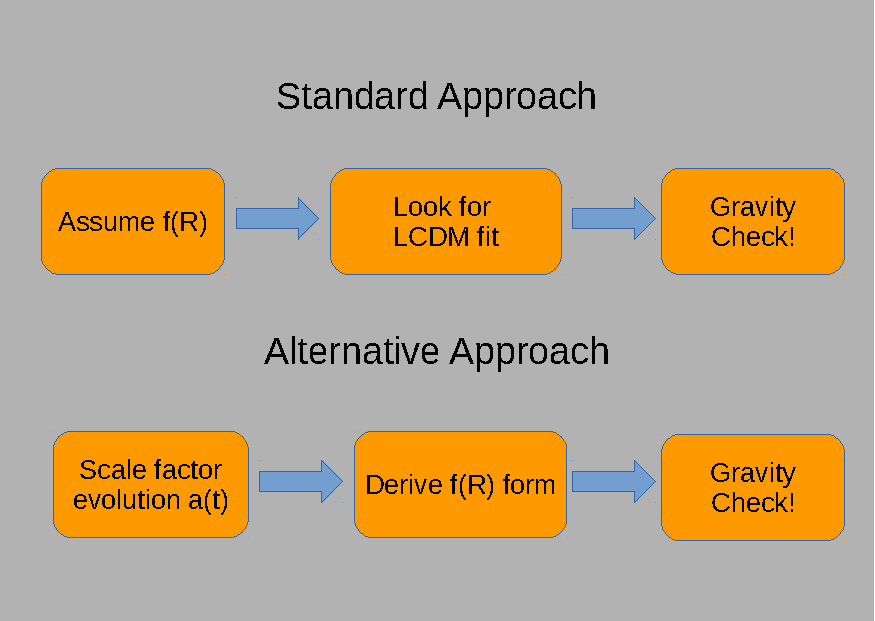
\includegraphics[width=0.8\linewidth]{IAGRG_poster_fR}
\caption{Approach for new `viable' $f(R)$}
\end{figure}

\end{block}

%----------------------------------------------------------------------------------------
%	CONCLUSION
%----------------------------------------------------------------------------------------

\begin{block}{Conclusions}

\begin{itemize}
\item Assuming a linearly coasting scale factor, we derived a potentially new `viable' forms of $f(R)$.
\item While some forms may look familar, they need to be re-evaluated in the light of linear coasting.
\item There are few options on constraining $f(R)$ models other than Cosmology
\begin{itemize}
	\item linear growth rate of structures
	\item gravitational weak lensing (\citet{tsujikawa2009dispersion})
	\item CMB and structure formation theories
	\item weak field limit from the solar system tests
	\item gravitational wave observations
\end{itemize}

\item These areas are to be explored in the subsequent work(s).
\end{itemize}

\end{block}

%----------------------------------------------------------------------------------------
%	REFERENCES
%----------------------------------------------------------------------------------------

\begin{block}{References}
        
\nocite{*} % Insert publications even if they are not cited in the poster
\small{\bibliographystyle{unsrt}
\bibliography{sample}}

\end{block}

%----------------------------------------------------------------------------------------
%	ACKNOWLEDGEMENTS
%----------------------------------------------------------------------------------------

\begin{block}{Acknowledgments}

\begin{itemize}
\item Nam mollis tristique neque eu luctus. Suspendisse rutrum congue nisi sed convallis. Aenean id neque dolor. Pellentesque habitant morbi tristique senectus et netus et malesuada fames ac turpis egestas.
\end{itemize}

\end{block}

%----------------------------------------------------------------------------------------
%	CONTACT INFORMATION
%----------------------------------------------------------------------------------------

\setbeamercolor{block title}{fg=black,bg=orange!70} % Change the block title color

\begin{block}{Contact Information}

\begin{itemize}
\item Web: \href{http://www.github.com/rohinkumar}{http://www.github.com/rohinkumar}
\item Email: \href{mailto:yrohinkumar@gmail.com}{yrohinkumar@gmail.com}
\item Phone: +91 9818092877
\end{itemize}

\end{block}

%----------------------------------------------------------------------------------------

\end{column} % End of the second column

\begin{column}{.015\textwidth}\end{column} % Empty spacer column

\end{columns} % End of all the columns in the poster

\end{frame} % End of the enclosing frame

\end{document}